% Abschlussarbeit am Ende der Oberschule
% Facharbeit zum parallelen Programmierparadigma
% Thomas Mittermair
% Oberschulzentrum J. Ph. Fallmerayer Brixen

\chapter{Parallele Programmierkonzepte, Anwendungsbeispiel und Vergleich}

	\section{Parallele Programmierkonzepte}
		\label{ParalleleProgrammierkonzepte}
	
		Seit der Entwicklung des parallelen Programmierparadigmas haben sich einige Konzepte und vor allem Programmiersprachen-Bibliotheken herausgebildet, wovon drei heute noch eingesetzte in diesem Kapitel erläutert werden sollen. Danach werden zwei dieser Technologien untereinander und auch mit reinen Prozessen und Threads anhand eines Anwendungsbeispiels verglichen.
		
		\subsection{MPI (Message Passing Interface)}
			\label{MPI}

			MPI, das \textit{Message Passing Interface}, wendet wie sich vom Namen bereits ableiten lässt das Message-Passing-Modell an. Dieses Modell geht davon aus, dass ein Parallelrechner mit verteiltem Speicher vorliegt, wobei jeder Prozess einen eigenen, lokalen Speicher besitzt. Da kein globaler Speicher in diesem Modell existiert, muss die Kommunikation zwischen den Prozessoren durch den Austausch von Nachrichten (Message-Passing) erfolgen. Um Daten vom lokalen Speicher eines Prozessors A in den eines anderen Prozessors B zu übertragen, muss A eine Nachricht an B senden, welche die Daten enthält. B muss die Nachricht dann empfangen und die Daten in einen Puffer, welcher im lokalen Speicher gespeichert wird, abspeichern.\\
			Um die Portabilität zu gewährleisten, werden keine Annahmen in Bezug auf das Verbindungsnetzwerk zwischen den Prozessoren gemacht. Jeder Prozessor kann mit jedem anderen Prozessor kommunizieren.\\
			Ein Programm, welches Message Passing verwendet, wird von einer Reihe von Prozessen ausgeführt, wobei jeder Prozess einen lokalen Speicher zur Verfügung hat und (im Optimalfall) auf einem eigenen Prozessor bzw. Prozessor-Kern läuft. Die Anzahl der beteiligten Prozesse wird meist beim Programmstart festgelegt. Jeder Prozess kann nun, analog zur zuvor erläuterten Funktionsweise, mit den lokalen Daten direkt arbeiten und mit den anderen Prozessen über das Senden und Empfangen von Nachrichten kommunizieren. Jeder Prozess kann dabei die selbe, aber auch verschiedene Aufgaben erfüllen.\\
			Den einzelnen Prozessen, die das Message-Passing-Programmm ausführen, müssen Kommunikationsoperationen zum Realisieren des Message-Passings zur Verfügung gestellt werden. Dies geschieht in der Regel durch eine Bibliothek einer Programmiersprache. Die Prozesse können dann auf die Funktionen, welche die Bibliothek bereitstellt, zugreifen.\\
			Eine solche Kommunikations-Bibliothek ist in der Regel hardwareunabhängig, weshalb sie auf verschiedensten Parallelrechnern genutzt werden können. Die bekannteste dieser Bibliotheken ist das MPI (\textit{Message Passing Interface}).\\
			MPI ist ein Standard zur Realisierung des Message-Passing-Modells. Es definiert die Syntax und Semantik von Funktionen, welche die Kommunikation und somit den Daten-Austausch ermöglichen. Die genaue Implementierung wird allerdings durch den Standard nicht festgelegt. Frei verfügbare Implementierungen sind beispielsweise MPICH, LAM/MPI oder auch OpenMPI (nicht zu verwechseln mit OpenMP, welches unter Kapitel \ref{OpenMP} erläutert wird).\\
			Diese Bibliothek wird für C, C++ und Fortran unterstützt. Der momentan aktuellste Standard ist MPI-3, welches 2012 erschienen ist. \cite{ParaProgRauber}
			
		\subsection{OpenMP (Open Multi-Processing)}
			\label{OpenMP}
			
			Der Standard OpenMP (\textit{Open Multi-Processing}) verfolgt einen etwas anderen Ansatz als MPI, da selbiger für Parallelrechner mit gemeinsamem Speicher ausgelegt ist. Die OpenMP-API\footnote{Eine API (\textit{Application Programming Interface}) ist eine Programmierschnittstelle, das heißt ein Programmteil, der anderen Programmen zur Anbindung an das System zur Verfügung gestellt wird. \cite{APIWikipedia}} stellt dabei eine Reihe von Compiler-Direktiven, Funktionen und Variablen zur Verfügung. Mit Hilfe dieser Compiler-Direktiven können die für gewöhnlich sequentiellen Programmiersprachen C, C++ und Fortran um Konstrukte zur parallelen Programmierung und auch zur Synchronisierung erweitert werden. Dabei kann sowohl lokaler, als auch gemeinsamer Speicher genutzt werden.\\
			Der erste OpenMP-Standard wurde im Jahre 1997 veröffentlicht und die Version 2.5 aus dem Jahr 2005 wird mittlerweile von den meisten Compilern unterstützt.\\
			Das Programmiermodell von OpenMP entspricht im Gegensatz zu dem von MPI auf zusammenarbeitenden Threads, welche parallel wiederum auf Prozessoren bzw. Prozessor-Kernen laufen. Die Erzeugung und Beendigung der Threads folgt dem unter Kapitel \ref{ForkJoinModell} vorgestellten Fork-Join-Modell. Wird ein OpenMP-Programm ausgeführt, so existiert zunächst nur genau ein Thread, welche \textit{Intial Thread} genannt wird. Somit erfolgt die Abarbeitung des Programmes sequentiell, bis das erste OpenMP-Konstrukt zur Parallelisierung gefunden wird. In diesem Schritt erzeugt der \textit{Intial Thread} eine Reihe von neuen Threads und bildet zusammen mit den neuen Threads ein Team, wobei der \textit{Intial Thread} zum \textit{Master Thread} befördert wird. Die Fork-Operation wird implizit durchgeführt, wird also vom Programmierer nicht direkt in die Wege geleitet. Der Programmcode innerhalb des parallelen Konstruktes wird \textit{parallele Region} genannt und wird vom gesamten Thread-Team ausgeführt. Jeder Thread kann dabei die selbe, aber auch verschiedene Aufgaben erfüllen. Am Ende der parallelen Region findet sich eine implizite Synchronisation und nur der Master Thread führt dann die Ausführung weiter, was einer impliziten Join-Operation entspricht. Parallele Regionen können auch verschachtelt werden, wobei jeder Thread, der auf ein OpenMP-Konstrukt zur Parallelisierung trifft, ein Team von Threads bildet und selbst zu einem \textit{Master Thread} wird.\\
			Das Speicher-Modell von OpenMP unterscheidet zwischen lokalem und gemeinsamem Speicher, wobei alle OpenMP-Threads auf den letztgenannten Speicher Zugriff haben. Um die unter Kapitel \ref{ProblemeParalleleBearbeitung} vorgestellten Probleme der Synchronisation wie beispielsweise zeitkritische Abläufe oder auch Deadlocks zu vermeiden, stellt der OpenMP-Standard auch Synchronisationsmechanismen in Form von Bibliotheksfunktionen zur Verfügung. Zusätzlich zu gemeinsame genutzten Variablen können die Threads auch private Variablen verwenden, welche nicht von anderen Threads zugegriffen werden können.\\
			Die Kompilierung eines OpenMP-Programmes führt zu einem Code, welcher Multithreading verwendet. \cite{ParaProgRauber} \cite{OpenMPWikipedia}

		\subsection{Cilk}
			\label{Cilk}
			
			Cilk, Cilk++ und Cilk Plus sind im Gegensatz zu MPI und OpenMP keine Standards, sondern eigene Programmiersprachen, welche für paralleles Rechnen unter Verwendung von Multithreading optimiert wurden. Die Syntax und Semantik ist an C und C++ angelehnt, weshalb diese Programmiersprachen als Erweiterungen von C bzw. C++ betrachtet werden können, welche das Parallelisieren von Schleifen und das Fork-Join-Modell, welche unter Kapitel \ref{ForkJoinModell} erläutert wurde, unterstützen.\\
			Die Programmiersprache Cilk wurde vom \textit{MIT Laboratory for Computer Science} entwickelt und 1994 veröffentlicht. Der Name \textit{Cilk} ist dabei eine Anspielung an Threads, welche Ausführungsfäden darstellen. Das englische Wort \textit{Silk}, welches mit \textit{(Seiden-) Faden} übersetzt werden kann, wurde so verändert, dass aus dem \textit{S} ein \textit{C} wurde, um auf die Programmiersprache C, auf welcher Cilk basiert, zu verweisen.\\
			Vor 2006 war Cilk nur auf Hochleistungsrechnen im professionellen Stil beschränkt und somit nicht verbreitet. Aus diesem Grund wurde das Unternehmen \textit{Cilk Arts} gegründet, welches die Programmiersprache Cilk modernisierte und somit kommerziell nutzbar machte. Die neue Version von Cilk wurde \textit{Cilk++} genannt und erschient 2008. Der Zusatz \textit{++} rührt daher, dass von nun an auch C++ unterstützt wurde.\\
			2009 gab Cilk Arts bekannt, von nun an Teil der \textit{Intel Corporation} zu sein. Bald darauf wurde Cilk++ zur aktuellen Version \textit{Intel Cilk Plus} erweitert. Selbige erschien im Jahre 2010.\\
			Das Konzept hinter Cilk besteht darin, dass der Programmierer dafür zuständig sein sollte, die Abschnitte im Code, die parallel verarbeitet werden können, zu identifizieren und mit den korrekten \textit{Cilk}-Schlüsselwörtern zu markieren. Er muss dann allerdings der Laufzeitumgebung die Aufgabe überlassen, wie die Arbeit genau auf die verfügbaren Prozessoren mit Hilfe von Threads aufgeteilt wird. Genau aus diesem Grund ist ein und dasselbe Cilk-Programm auf einem Ein-, aber auch auf einem \textit{n}-Prozessor-System lauffähig, ohne Veränderungen im Quellcode tätigen zu müssen.\\
			Im Folgenden werden die wichtigsten beiden Schlüsselwörter, um die Cilk Plus die Programmiersprache C erweitert, erläutert. Dabei handelt es sich um die beiden Wörter \textit{spawn} (zu Deutsch \textit{vermehren}), und \textit{sync} (in Anlehnung an \textit{Synchronisierung}). Beide werden in Zusammenhang mit der Realisierung des unter Kapitel \ref{ForkJoinModell} erwähnten Fork-Join-Modell benötigt. Das \textit{spawn}-Schlüsselwort wird einem Funktionsaufruf vorangestellt (beispielsweise \textit{spawn f(x)}). Das bedeutet, dass die Anweisungen innerhalb der Funktion \textit{f(x)} problemlos parallel zu den auf den Funktionsaufruf folgenden Anweisungen ausgeführt werden kann. Der Scheduler ist allerdings nicht gezwungen, diesen Code dann tatsächlich parallel auszuführen. Dieses Schlüsselwort kann also eher als eine \textit{Empfehlung der parallelen Verarbeitung} betrachtet werden. Dieses Schlüsselwort realisiert also einen Fork. Das \textit{sync}-Schlüsselwort ist das Gegenstück zu \textit{spawn}. Es weist den Compiler darauf hin, dass die Ausführung der darauf folgenden Anweisungen erst vollzogen werden kann, sobald alle zuvor mit Hilfe des Schlüsselworts \textit{spawn} parallel ausgeführten Funktionen vollständig abgearbeitet worden sind. Somit wird durch dieses Schlüsselwort ein Join realisiert. \cite{CilkWikipedia}

	\section{Anwendungsbeispiel und Vergleich der parallelen Programmierkonzepte}

		Einige der im Rahmen dieser Arbeit vorgestellten Konzepte zur parallen Programmierung, nämlich Prozesse, Threads, MPI und OpenMP werden nun anhand eines praktischen Anwendungsbeispiels verglichen.\\
		Dabei handelt es sich um die Berechnung der Primzahlen zwischen 1 und 100.000. Dies ist eine rechenaufwändige Aufgabe, die durch Parallelisierung (erheblich) optimiert werden kann.
		
		\subsection{Voraussetzungen}
			
			Alle im Folgenden vorgestellten Programme und Messdaten wurden auf einem Ubuntu-System (Ubuntu 16.04 LTS) ausgeführt, welches wiederum in einer virtuellen Maschine (VMware Workstation 14 Player) arbeitete. Das virtuelle Ubuntu-System war dabei wie folgt konfiguriert:
			
			\begin{itemize}
				\item Speicherplatz des Hauptspeichers: 15,6 GiB
				\item Prozessor: Intel Core i7-6700HQ CPU @ 2.60GHz x 4
				\item Typ des Betriebssystems: 64 Bit
				\item Speicherplatz des Sekundärspeichers: 88,6 GB
			\end{itemize}
		
			Während der Berechnungen wurde zusätzlich die Netzwerk-Verbindung deaktiviert, um das Herunterladen von Updates und Ähnlichem im Hintergrund, was die Messdaten verfälschen hätte können, zu verhindern.
		
		\subsection{Programmierung und Auswertung}
		
			Nun werden die verschiedenen Ansätze zur Realisierung des Programmes zur Primzahlen-Berechnung vor allem anhand der Messdaten verglichen.\\
			Dabei ist anzumerken, dass alle Messungen 50 Mal durchgeführt wurden und aus diesen Messergebnissen jeweils immer der Median gebildet wurde, um Ausreiser zu eliminieren und vertrauenswürdige Messergebnisse zu erzielen. Des Weiteren sind alle x-Achsen der im Folgenden dargestellten Diagramme logarithmisch (zur Basis 2) skaliert, das bedeutet, dass die auf der x-Achse aufgetragenen Werte exponentiell (zur Basis 2) und nicht linear erhöht werden.
		
			\subsubsection{Sequentielle Lösung}
			
				Die Primzahlen wurden zunächst mit einem sequentiellen Algorithmus berechnet und die Laufzeit gemessen. Die sequentielle Lösung stellt die einfachste, aber auch die s(abgesehen von MPI) langsamste Lösung zur Berechnung von Primzahlen dar. Dabei wird jede Zahl von 1 bis 100.000 nacheinander überprüft und festgestellt, ob es sich bei der jeweiligen Zahl um eine Primzahl handelt oder nicht. Es findet keinerlei Parallelisierung statt.\\
				Der Median der Laufzeit des sequentiellen Algorithmuses beträgt 12,84 s. Diese Größe ist alleinstehend nicht aussagekräftig, sondern wird erst beim Vergleich mit den parallelen Programmierkonzepten interessant.
			
			\subsubsection{Parallele Lösungen}
			
				Nun werden die verschiedenen parallelen Lösungsmöglichkeiten für die Berechnung der Primzahlen aufgezeigt und verglichen.
				
				\begin{description}
					
					\item[Parallele Lösung des Problems durch Prozesse]
					
						Zunächst wurde versucht, das gegebene Problem durch Prozesse, also dem Grundkonzept der parallelen Programmierung, zu lösen, welches bereits unter Punkt \ref{ProzessModell} erläutert wurde. In diesem Fall wurden UNIX-Prozesse verwendet.\\
						Dabei werden die Zahlen von 1 bis 100.000 abhängig von der Anzahl der verwendeten Prozesse $P$ in $P$ möglichst gleich große Intervalle aufgeteilt, um das unter Kapitel \ref{Lastenverteilung} erwähnte Load Balancing zu gewährleisten.\\
						Das Programm funktioniert dabei wie folgt: Zunächst wird ein einziger Prozess zur Lösung des Problems verwendet. Dann werden die Primzahlen mit diesem einen Prozess 50 Mal berechnet und die Laufzeit gemessen, um anschließend wiederum den Median bilden zu können. Im Anschluss wird die Anzahl der Prozesse erhöht und dasselbe wieder durchgeführt.\\
						Die Anzahl der Prozesse steigt dabei nicht ständig gleich schnell an, sondern lässt sich durch die folgende Funktion $P(n)$ angeben. $P$ ist dabei die Anzahl der verwendeten Prozesse im $n$. Durchlauf, wobei wie bereits erwähnt jeder Durchlauf nochmals 50 Mal unter gleichen Bedingungen wiederholt wird, um Ausreiser in der Zeitmessung zu eliminieren, und in jedem Durchlaufs-Wechsel die Anzahl der Prozesse erhöht wird.
						
						\begin{equation}
							P(n) =
							\begin{cases}
								P(n - 1) + 1 & \text{für } 1 \leq P_n < 10\\
								P(n - 1) + 2 & \text{für } 10 \leq P_n < 50\\
								P(n - 1) + 50 & \text{für } 50 \leq P_n < 1000\\
								P(n - 1) + 1000 & \text{für } P_n \geq 1000\\
							\end{cases}
						\end{equation}
						
						Als Start-Wert gilt $P(1) = 1$.\\
						Um den Prozessen, welche am Problem gemeinsam arbeiten, und grundsätzlich über vollkommen getrennte Speicherbereiche verfügen, eine Kommunikation zu ermöglichen, wurde ein gemeinsamer Speicher für alle beteiligten Prozesse eingerichtet, wobei der Zugriff darauf mit Hilfe einer Semaphore geregelt wurde, die jeweils nur einen Prozess gleichzeitig in den kritischen Bereich eintreten ließ.\\
						Durch Ausloten der Grenzen auf dem verwendeten System wurde festgestellt, dass sich maximal 11.000 Prozesse erzeugen lassen. Deshalb befindet sich im Rahmen dieses Versuches $P(n)$ immer im Intervall $1 \leq P(n) \leq 11.000$.
						Die Messdaten werden auf Grund des großen Umfangs im Rahmen der Arbeit nicht direkt aufgelistet, sondern aus der Anzahl der verwendeten Prozesse und dem dazugehörigen Laufzeit-Median wurde der Speedup, welcher in Kapitel \ref{Speedup} erläutert wurde, und auch die Effizienz, die unter Punkt \ref{Effizienz} eingeführt wurde, ermittelt. Diese beiden wichtigen Kennzahlen wurden dann in zwei Diagrammen dargestellt.\\
						Der Speedup $S_P$ wurde in Abhängigkeit von der Anzahl der verwendeten Prozesse $P$ berechnet und grafisch dargestellt, was in Abbildung \ref{fig:Speedup_Prozesse} erkenntlich ist.
						
						\begin{figure}
							\centering	
							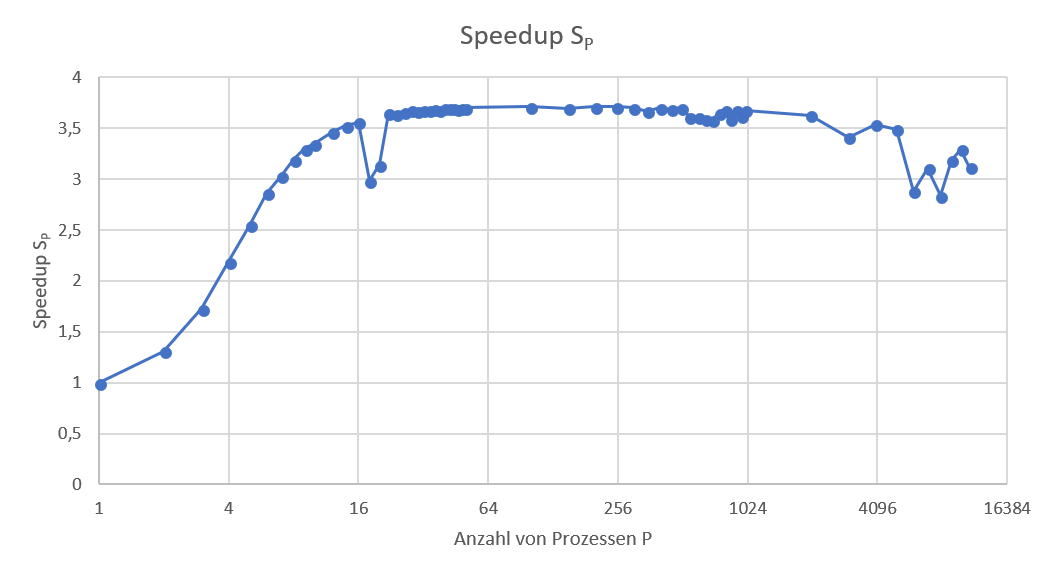
\includegraphics[width=11cm]{Abbildungen/Speedup_Prozesse.png}
							\caption{Grafische Darstellung des Zusammenhangs zwischen dem Speedup und der Anzahl der verwendeten Prozesse.}
							\label{fig:Speedup_Prozesse}
						\end{figure}
					
						Aus dem gegebenen Diagramm lassen sich einige Informationen gewinnen. Mit einem Prozess ergibt sich ein Speedup von genau 1, was auch nachvollziehbar sein sollte. Bei steigender Anzahl von Prozessen steigt zunächst auch der Speedup, allerdings zeigt sich ab 16 Prozessen (von zwei Ausreisern abgesehen) keine signifikante Veränderung des Speedups mehr. Es scheint laut Diagramm auch eine obere Schranke für den Speedup zu existieren, die sich im Bereich zwischen 3,5 und 4 bewegt. Ab ca. 1000 Prozessen ist erkenntlich, dass der Verwaltungsaufwand für die Prozesse sogar den Mehrwert an Rechenleistung, der mit der Erhöhung der Anzahl der Prozesse einhergeht, übersteigt, weshalb der Speedup von diesem Punkt an zu sinken beginnt, wobei die Werte allerdings Schwankungen aufweisen. Ein Abwärtstrend ist aber erkenntlich.\\
						Bemerkenswert ist vor allem die Tatsache, dass die Messungen auf einem System mit einem 4-Kern-Prozessor ausgeführt wurden und man meinen möchte, dass ab 4 Prozessen, also einem Prozess pro Kern, keine Speedup-Steigerung mehr möglich sein sollte. In der Tat ist dies allerdings nicht der Fall. Höchstwahrscheinlich ist dies im Scheduling-Algorithmus des Systems begründet. Bis zu einem gewissen Grad ermöglicht die Erhöhung der Anzahl der Prozesse, dass der Scheduler insgesamt dem gesamten Programm (also allen Prozessen zusammen) mehr CPU-Zeit zur Verfügung stellt als nur den 4 Prozessen.\\
						In der Praxis muss allerdings nicht nur der Geschwindigkeitsgewinn, sondern auch die Effizienz der Lösung betrachtet werden. Selbige ist in Abbildung \ref{fig:Effizienz_Prozesse} dargestellt.
						
						\begin{figure}
							\centering	
							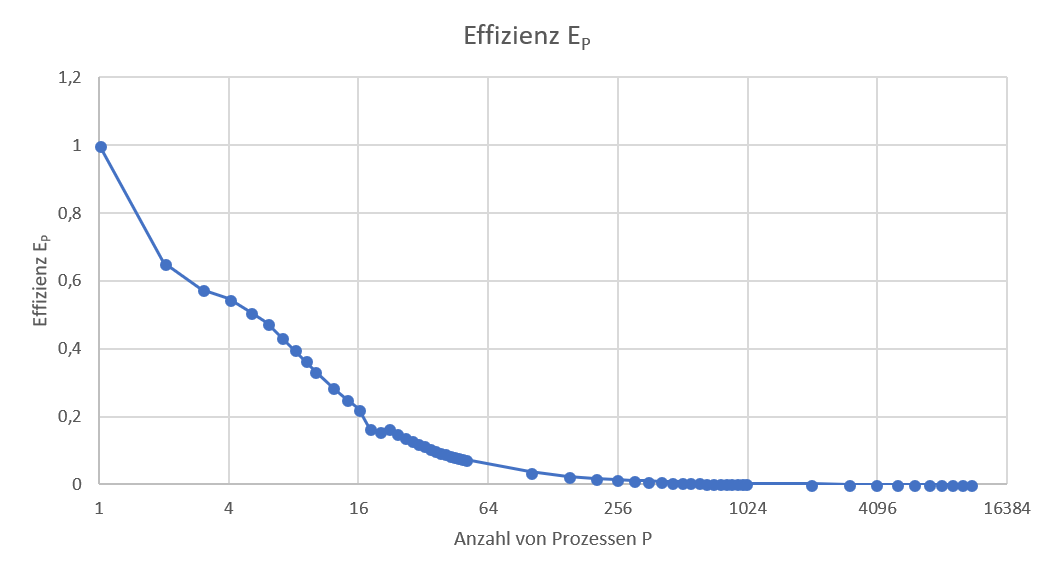
\includegraphics[width=11cm]{Abbildungen/Effizienz_Prozesse.png}
							\caption{Grafische Darstellung des Zusammenhangs zwischen der Effizienz und der Anzahl der verwendeten Prozesse.}
							\label{fig:Effizienz_Prozesse}
						\end{figure}
						
						Die Effizienz entspricht in diesem Fall einer stetig sinkenden Funktion, welche zu Beginn drastisch sinkt und sich dann asymptotisch 0 annähert. Auch ist erkenntlich, dass die Effizienz bis ca. 16 Prozessen, wie auch aus dem Speedup-Diagramm hervorgeht, akzeptable Werte zwischen 100\% und 20\% annimmt, während sie nachher immer weiter sinkt und schließlich annähernd 0\% wird.
					
					\item[Parallele Lösung des Problems durch Threads]
						
						Nun wurde das Problem mit Hilfe von Threads, also einem weiteren wichtigen Grundbaustein der parallelen Programmierung, gelöst, welcher bereits unter Punkt \ref{ThreadModell} erläutert wurde. In diesem Fall wurden POSIX-Threads verwendet.\\
						Das Programm läuft dabei ähnlich zum Vorherigen mit Prozessen ab, auch die Erhöhung der Anzahl der Threads $T$ wurde nach dem selben Schema vollzogen. Allerdings war in diesem Fall kein gemeinsamer Speicher nötig, weil sich die Threads den gemeinsamen Speicher des Prozesses, zu welchem sie gehören, teilen. In diesem Fall wurde keine Semaphore zur Synchronisation benötigt, da zwar gemeinsame Ressourcen existierten, die Threads sich jedoch nie in die Quere kommen konnten. Die Funktion, die die Anzahl der Threads $T$ in Abhängigkeit vom Durchlauf $n$ angibt, nennt sich in diesem Fall $T(n)$.
						Durch Austesten der Grenzen auf dem verwendeten System wurde in diesem Fall festgestellt, dass sich maximal 32.000 Threads erzeugen lassen. Deshalb befindet sich im Rahmen dieses Versuches $T(n)$ immer im Intervall $1 \leq T(n) \leq 32.000$.
						Die Messdaten werden auf Grund des großen Umfangs im Rahmen der Arbeit wieder nicht direkt aufgelistet, sondern aus der Anzahl der verwendeten Threads und dem dazugehörigen Laufzeit-Median wurde wieder der Speedup, welcher in Kapitel \ref{Speedup} erläutert wurde, und auch die Effizienz, die unter Punkt \ref{Effizienz} eingeführt wurde, ermittelt. Diese beiden wichtigen Kennzahlen wurden dann in zwei Diagrammen dargestellt.\\
						Der Speedup $S_T$ wurde in Abhängigkeit von der Anzahl der verwendeten Threads $T$ berechnet und grafisch dargestellt, was in Abbildung \ref{fig:Speedup_Threads} erkenntlich ist.
						
						\begin{figure}
							\centering	
							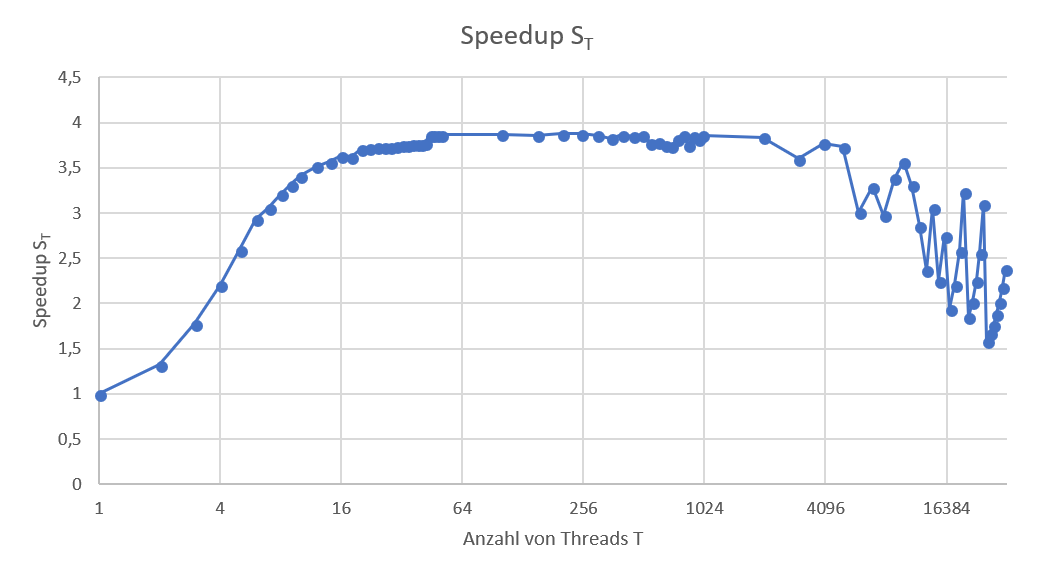
\includegraphics[width=11cm]{Abbildungen/Speedup_Threads.png}
							\caption{Grafische Darstellung des Zusammenhangs zwischen dem Speedup und der Anzahl der verwendeten Threads.}
							\label{fig:Speedup_Threads}
						\end{figure}
						
						Aus dem gegebenen Diagramm lassen sich ähnliche Erkenntnisse wie aus der Abbildung \ref{fig:Speedup_Prozesse} gewinnen. Auch in diesem Fall zeigt sich eine allmähliche Erreichung der oberen Schranke des Speedups bei ca. 16 Threads. Danach zeigt sich keine signifikante Verbesserung des Speedups mehr. Die obere Schranke für den Speedup bewegt sich auch hier im Bereich zwischen 3,5 und 4. Ab ca. 1000 Threads ist erkenntlich, dass der Verwaltungsaufwand für die Threads sogar den Nutzen, der mit der Erhöhung der Anzahl der Threads einhergeht, übersteigt, weshalb der Speedup von diesem Punkt an zu sinken beginnt, wobei die Werte allerdings Schwankungen aufweisen.\\
						Bemerkenswert ist auch hier die schon bei Prozessen genannte Tatsache, dass die Messungen auf einem System mit einem 4-Kern-Prozessor ausgeführt wurden und man meinen möchte, dass ab 4 Prozessen, also einem Prozess pro Kern, keine Speedup-Steigerung mehr möglich sein sollte. In der Tat ist dies allerdings nicht der Fall. Die möglichen Gründe hierfür sind mit jenen bei Verwendung von Prozessen ident.\\
						Nun wird die Effizienz betrachtet. Sie ist in Abbildung \ref{fig:Effizienz_Threads} dargestellt.
						
						\begin{figure}
							\centering	
							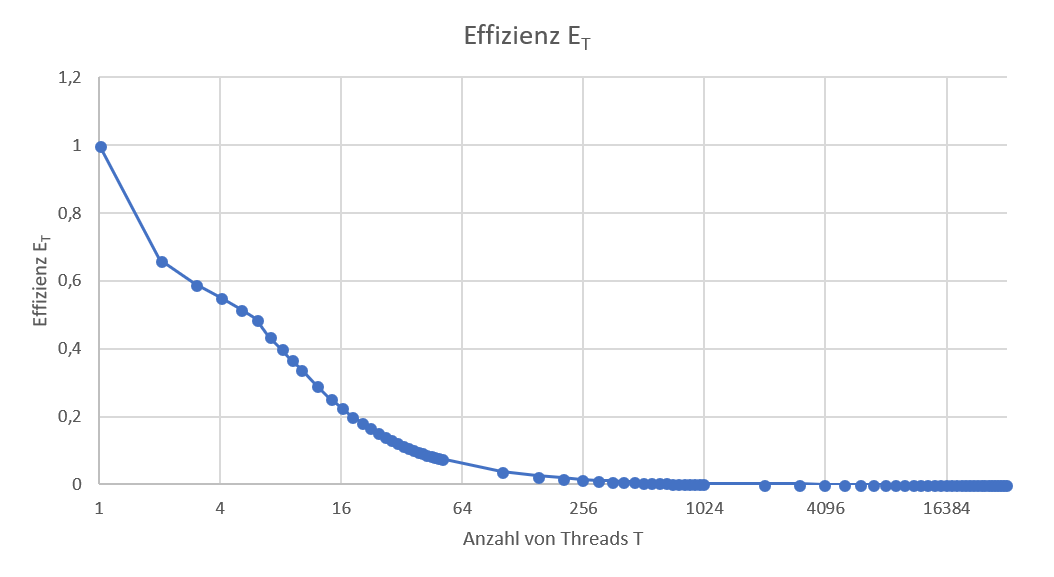
\includegraphics[width=11cm]{Abbildungen/Effizienz_Threads.png}
							\caption{Grafische Darstellung des Zusammenhangs zwischen der Effizienz und der Anzahl der verwendeten Threads.}
							\label{fig:Effizienz_Threads}
						\end{figure}
						
						Die Effizienz kommt auch in diesem Fall einer stetig sinkenden Funktion gleich, welche zu Beginn drastisch sinkt und sich dann asymptotisch 0 annähet. Auch ist erkenntlich, dass die Effizienz bis ca. 16 Threads, wie auch aus dem Speedup-Diagramm hervorgeht, akzeptable Werte zwischen 100\% und 20\% annimmt, während sie nachher immer weiter sinkt und schließlich annähernd 0\% wird.

					\item[Parallele Lösung des Problems durch MPI]
					
						Nun wurde eine der unter Kapitel \ref{ParalleleProgrammierkonzepte} genannten Technologien, nämlich MPI, das \textit{Message Passing Interface}, angewendet, um die Primzahlen-Berechnung durchzuführen. Folglich wurden MPI-Prozesse verwendet.\\
						Dabei werden die Zahlen von 1 bis 100.000 abhängig von der Anzahl der verwendeten MPI-Prozesse $P$ in $P$ möglichst gleich große Intervalle aufgeteilt, um erneut das unter Kapitel \ref{Lastenverteilung} erwähnte Load Balancing zu gewährleisten.\\
						Das Programm funktioniert dabei wie folgt: Zunächst werden zwei Prozesse zur Lösung des Problems verwendet. Ein Prozess ist dabei stets der Master-Prozess, der die Aufteilung koordiniert und selbst keine Berechnungen durchführt, während der andere Prozess die Berechnungen durchführt. Dann werden die Primzahlen mit diesem einen Prozess 50 Mal berechnet und die Laufzeit gemessen, um anschließend wiederum den Median bilden zu können. Im Anschluss wird die Anzahl der Prozesse erhöht und dasselbe wieder durchgeführt.\\
						Die Anzahl der Prozesse steigt dabei nicht ständig gleich schnell an, sondern lässt sich durch die folgende Funktion $P(n)$ angeben. Diese Funktion ist im Vergleich zu den vorher vorgestellten Lösungen anders, weil mit MPI auf dem vorhandenen System nur maximal 253 MPI-Prozesse erzeugt werden konnten. $P$ ist dabei die Anzahl der verwendeten MPI-Prozesse im $n$. Durchlauf, wobei wie bereits erwähnt jeder Durchlauf nochmals 50 Mal unter gleichen Bedingungen wiederholt wird, um Ausreiser in der Zeitmessung zu eliminieren, und in jedem Durchlaufs-Wechsel die Anzahl der Prozesse erhöht wird.
						
						\begin{equation}
							P(n) =
							\begin{cases}
								P(n - 1) + 1 & \text{für } 1 \leq P_n < 10\\
								P(n - 1) + 2 & \text{für } 10 \leq P_n < 50\\
								P(n - 1) + 10 & \text{für } 50 \leq P_n < 100\\
								P(n - 1) + 50 & \text{für } P_n \geq 100\\
							\end{cases}
						\end{equation}
						
						Als Start-Wert gilt $P(1) = 1$.\\
						Um den Prozessen, welche am Problem gemeinsam arbeiten, und grundsätzlich über vollkommen getrennte Speicherbereiche verfügen, eine Kommunikation zu ermöglichen, wurden die Kommunikations-Funktionen zum Senden und Empfangen von Daten, welche von der MPI-Bibliothek zur Verfügung gestellt werden, verwendet. Da keine gemeinsame Ressource existierte, war keine Synchronisierung von Nöten.\\
						Durch Ausloten der Grenzen auf dem verwendeten System wurde wie bereits angedeutet festgestellt, dass sich maximal 253 Prozesse erzeugen lassen. Deshalb befindet sich im Rahmen dieses Versuches $P(n)$ immer im Intervall $1 \leq P(n) \leq 253$.
						Die Messdaten werden wieder auf Grund des großen Umfangs im Rahmen der Arbeit nicht direkt aufgelistet, sondern aus der Anzahl der verwendeten MPI-Prozesse und dem dazugehörigen Laufzeit-Median wurde der Speedup, welcher in Kapitel \ref{Speedup} erläutert wurde, und auch die Effizienz, die unter Punkt \ref{Effizienz} eingeführt wurde, ermittelt. Diese beiden wichtigen Kennzahlen wurden nun in zwei Diagrammen dargestellt.\\
						Der Speedup $S_P$ wurde in Abhängigkeit von der Anzahl der verwendeten MPI-Prozesse $P$ berechnet und grafisch dargestellt, was in Abbildung \ref{fig:Speedup_MPI} erkenntlich ist.
						
						\begin{figure}
							\centering	
							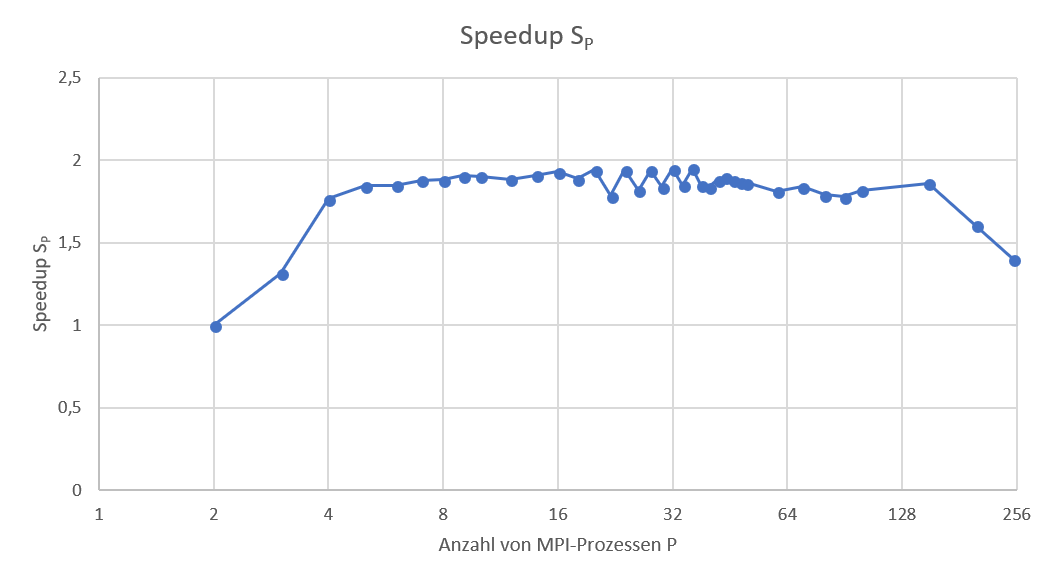
\includegraphics[width=11cm]{Abbildungen/Speedup_MPI.png}
							\caption{Grafische Darstellung des Zusammenhangs zwischen dem Speedup und der Anzahl der verwendeten MPI-Prozesse.}
							\label{fig:Speedup_MPI}
						\end{figure}
						
						Aus dem gegebenen Diagramm lassen sich einige Informationen gewinnen, die sich jedoch von den bisherigen Ergebnissen, welche mit den anderen Technologien erzielt wurden, unterscheiden. Mit zwei Prozessen ergibt sich ein Speedup von genau 0,5, was auch nachvollziehbar sein sollte, da ein Prozess dem Master entspricht und nur der zweite Prozess, der Slave, tatsächlich Arbeit verrichtet. Bei steigender Anzahl von MPI-Prozessen steigt zunächst auch der Speedup stark an, allerdings zeigt sich ab 4 MPI-Prozessen eine signifikante Verbesserung des Speedups mehr. Es scheint laut Diagramm auch eine obere Schranke für den Speedup zu existieren, die sich im Bereich zwischen 1,5 und 2 bewegt. Ab ca. 130 MPI-Prozessen ist erkenntlich, dass der Verwaltungsaufwand für die Prozesse sogar den Nutzen, der mit der Erhöhung der Anzahl der Prozesse einhergeht, übersteigt, weshalb der Speedup von diesem Punkt an zu sinken beginnt.\\
						Bemerkenswert ist vor allem die Tatsache, dass die Messungen auf einem System mit einem 4-Kern-Prozessor ausgeführt wurden und im Gegenteil zu den bis jetzt erzielten Ergebnissen ab ca. 4 Prozessen keine Speedup-Steigerung mehr möglich ist.\\
						In der Praxis muss allerdings nicht nur der Geschwindigkeitsgewinn, sondern auch die Effizienz der Lösung betrachtet werden. Selbige ist in Abbildung \ref{fig:Effizienz_MPI} dargestellt.
						
						\begin{figure}
							\centering	
							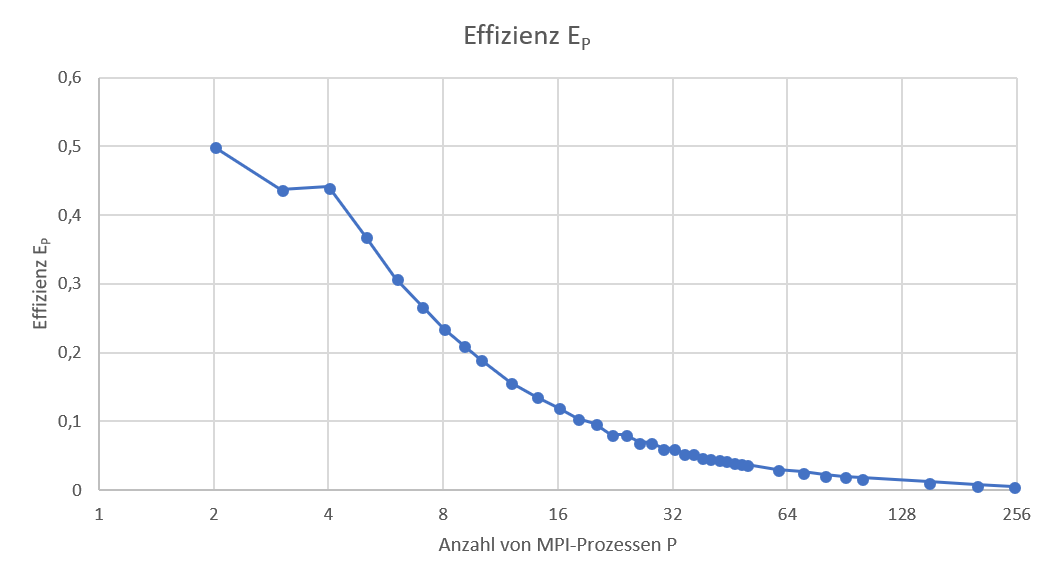
\includegraphics[width=11cm]{Abbildungen/Effizienz_MPI.png}
							\caption{Grafische Darstellung des Zusammenhangs zwischen der Effizienz und der Anzahl der verwendeten MPI-Prozesse.}
							\label{fig:Effizienz_MPI}
						\end{figure}
						
						Die Effizienz entspricht in diesem Fall nicht einer stetig sinkenden Funktion, sondern vom Übergang von 3 auf 4 MPI-Prozessen steigt die Effizienz sogar minimal an, befindet sich bei ca. 45\%. Ab dem Erreichen von 4 MPI-Prozessen, also der Grenze, ab welcher die Anzahl der MPI-Prozessen gleich der Anzahl der vorhandenen Prozessor-Kerne ist, beginnt die Funktion sehr schnell zu sinken und schließlich annähernd 0\% wird.
						
					\item[Parallele Lösung des Problems durch OpenMP]
					
						Nun wurde das Problem mit Hilfe der zweiten der unter Kapitel \ref{ParalleleProgrammierkonzepte} genannten Technologien, OpenMP, also dem \textit{Open Multi-Processing}, gelöst. Aus diesem Grund wurden OpenMP-Threads verwendet.\\
						Das Programm läuft dabei ähnlich zum Vorherigen, welches normale Threads verwendet, ab, auch die Erhöhung der Anzahl der OpenMP-Threads $T$ wurde nach dem selben Schema vollzogen. Auch war in diesem Fall kein gemeinsamer Speicher nötig, weil sich die Threads den gemeinsamen Speicher des Prozesses, zu welchem sie gehören, teilen. In diesem Fall wurde keine Semaphore zur Synchronisation benötigt, da zwar gemeinsame Ressourcen existierten, die OpenMP-Threads sich jedoch nie in die Quere kommen konnten. Die Funktion, die die Anzahl der OpenMP-Threads $T$ in Abhängigkeit vom Durchlauf $n$ angibt, nennt sich in diesem ebenfalls Fall $T(n)$.\\
						Durch Ausloten der Grenzen auf dem verwendeten System wurde in diesem Fall festgestellt, dass sich maximal 11.000 OpenMP-Threads erzeugen lassen. Deshalb befindet sich im Rahmen dieses Versuches $T(n)$ immer im Intervall $1 \leq T(n) \leq 11.000$.
						Die Messdaten werden auf Grund des großen Umfangs im Rahmen der Arbeit wieder nicht direkt aufgelistet, sondern aus der Anzahl der verwendeten OpenMP-Threads und dem dazugehörigen Laufzeit-Median wurde wieder der Speedup, welcher in Kapitel \ref{Speedup} erläutert wurde, und auch die Effizienz, die unter Punkt \ref{Effizienz} eingeführt wurde, ermittelt. Diese beiden wichtigen Kennzahlen wurden dann wieder in zwei Diagrammen dargestellt.\\
						Der Speedup $S_T$ wurde in Abhängigkeit von der Anzahl der verwendeten OpenMP-Threads $T$ berechnet und grafisch dargestellt, was in Abbildung \ref{fig:Speedup_OpenMP} erkenntlich ist.
						
						\begin{figure}
							\centering	
							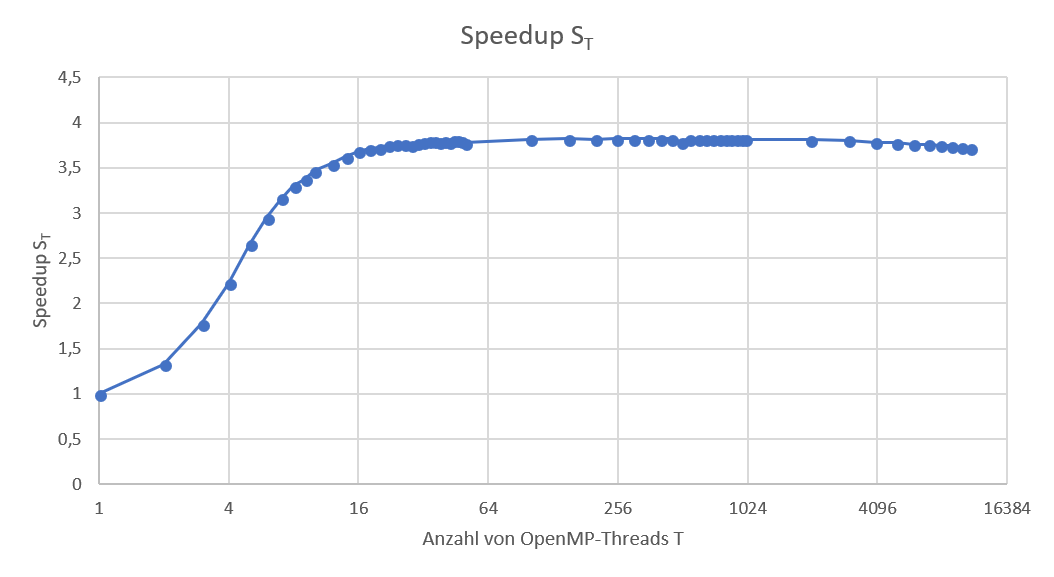
\includegraphics[width=11cm]{Abbildungen/Speedup_OpenMP.png}
							\caption{Grafische Darstellung des Zusammenhangs zwischen dem Speedup und der Anzahl der verwendeten OpenMP-Threads.}
							\label{fig:Speedup_OpenMP}
						\end{figure}
						
						Aus dem gegebenen Diagramm lassen sich ähnliche Erkenntnisse wie aus der Abbildung \ref{fig:Speedup_Threads} gewinnen. Auch in diesem Fall zeigt sich eine allmähliche Erreichung der oberen Schranke des Speedups bei ca. 16 Threads. Danach lässt sich keine signifikante Verbesserung des Speedups mehr feststellen. Die obere Schranke für den Speedup bewegt sich auch in diesem Fall im Bereich zwischen 3,5 und 4. Allerdings ist, da maximal 11.000 Threads erzeugt wurden, nur ein geringer Abwärtstrend bei sehr vielen OpenMP-Threads erkenntlich, was bedeutet, dass zumindest bei dem im Rahmen dieses Versuches untersuchten Verhalten der Verwaltungsaufwand für die OpenMP-Threads kaum den Nutzen, der mit der Erhöhung der Anzahl der OpenMP-Threads einhergeht, übersteigt, weshalb der Speedup bei ca. 4.000 OpenMP-Threads nur geringfügig zu sinken beginnt.\\
						Bemerkenswert ist auch hier die schon bei Prozessen genannte Tatsache, dass die Messungen auf einem System mit einem 4-Kern-Prozessor ausgeführt wurden und man meinen möchte, dass ab 4 OpenMP-Threads, also einem OpenMP-Thread pro Kern, keine Speedup-Steigerung mehr möglich sein sollte. In der Tat ist dies allerdings nicht der Fall. Die möglichen Gründe hierfür sind mit jenen bei Verwendung von Threads ident.\\
						Die Speedup-Kurve weist einen sehr regelmäßigen Verlauf auf und scheint im gegebenen Intervall einem \textit{Sättigungsvorgang} gleichzukommen. Dabei nähert sich eine wachsende Größe einem konstanten Endwert an. Diese Annäherung erfolgt dabei asymptotisch, das bedeutet, dass der Endwert in der Theorie nie erreicht werden kann. Es existieren mehrere Arten von Sättigungsvorgängen, wobei der in diesem Fall ersichtliche Graph ein logistisches Wachstum aufzuweisen scheint. Dies ist ein Spezialfall des exponentiellen Wachstums.\\
						Mathematisch betrachtet können logistische Wachstumsvorgänge durch Funktionen der folgenden Form beschrieben werden:
						
						\[
							f(x) = \frac{f(0) \cdot s}{f(0) + (s - f(0)) \cdot e^{-s \cdot k \cdot x}}
						\]
						
						Dabei ist $f(x)$ der Wert der logistisch wachsenden Größe an der Stelle $x$, wobei $x$ oft ein Zeitpunkt und $f(x)$ somit meist eine zeitabhängige Größe ist. $f(0)$ ist der Anfangswert an der Stelle 0, also der Ausgangswert der wachsenden Größe. $s$ ist der Grenzwert der Funktion für beliebig große Werte von $x$, also die sogenannte \textit{Sättigungsgrenze}. Diesen Wert kann die Funktion niemals überschreiten und nur im Unendlichen erreichen. \cite{MathematikTechnischeAnwendungen2} \cite{LogistischesWachstum}\\		
						Nun wird versucht, den Graph aus Abbildung \ref{fig:Speedup_OpenMP} durch eine Funktion der obigen Form zu beschreiben bzw. anzunähern.\\
						Mit Hilfe der Abbildung bzw. den Messergebnissen ließe sich eine Größe direkt herausfinden, nämlich $s$. Es gilt $s \approx 3,82$. Der Wert von $s$ ist dabei gerundet, weil sich kein exakter Wert aus den Messergebnissen ergibt. Für die Angabe der Funktionsgleichung des logistischen Wachstums fehlt nun aber noch der konstante Faktor $k$ und der Funktionswert an der Stelle 0, also $f(0)$. Das Problem ist hierbei, dass $f(0)$ aus den Werten nicht bestimmt werden kann, da die Messwerte bei 1 OpenMP-Thread beginnen.\\
						Aus diesem Grund muss auf eine andere Darstellungsform des logistischen Wachstums, nämlich die \textit{rekursive Form}, zurückgegriffen werden. Diese schaut allgemein wie folgt aus.
						
						\begin{align*} 
							f(x + 1) = f(x) + d \cdot f(x) \cdot (s - f(x))
						\end{align*}
						
						Dabei ist $f(x)$ der Funktionswert an der Stelle $x$ und $f(x + 1)$ der Funktionswert nach einem weiteren Schritt. $d$ ist ein konstanter Faktor und $s$ ist wieder die Sättigungsgrenze. Anzumerken ist hier, dass auf Grund der rekursiven Darstellung nur diskrete Werte für $x$ eingesetzt werden können, die sich im Abstand von 1 befinden. Des Weiteren ist die Angabe eines Startwerts notwendig. \cite{LogistischesWachstumRekursiv}\\
						Nun muss der Faktor $d$ bestimmt werden. Zuvor werden allerdings noch die Bezeichnungen verändert. $f(x)$ wird im Folgenden mit $S(T)$ bezeichnet, da diese Funktion den Zusammenhang zwischen dem Speedup $S$ und der Anzahl von verwendeten OpenMP-Threads $T$ beschreibt.\\
						Um $d$ zu bestimmen werden zwei Punkte benötigt, durch welche der Graph des Speedups verläuft, wobei die Distanz dieser beiden Punkte in x-Richtung genau 1 sein muss. Aus der Abbildung bzw. den Messwerten lässt sich feststellen, dass zwei solche Punkte z.B. $Q(4 | 2,222)$ und $R(5 | 2,657)$ sind. Des Weiteren wird der Wert der Sättigungsgrenze benötigt, welcher wie bereits beschrieben $s \approx 3,82$ beträgt.

						\begin{align*}
							f(x + 1) = f(x) + d \cdot f(x) \cdot (s - f(x))\\
							S(T + 1) = S(T) + d \cdot S(T) \cdot (s - S(T))\\
							S(T + 1) = S(T) + d \cdot S(T) \cdot (3,82 - S(T))
						\end{align*}
						
						Nun werden die beiden Punkt $Q$ und $R$ eingesetzt.
						
						\begin{align*}
							S(T + 1) = S(T) + d \cdot S(T) \cdot (3,82 - S(T))\\
							2,657 = 2,222 + d \cdot 2,222 \cdot (3,82 - 2,222)\\
							2,657 = 2,222 + d \cdot 2,222 \cdot 1,598
						\end{align*}
						
						Löst man diese Gleichung, so kommt man zum folgenden Wert für den Faktor $d$.
						
						\begin{align*}
							d = \frac{2,657 - 2,222}{2,222 \cdot 1,598} \approx 0,1225
						\end{align*}
						
						Nun kann $d\approx 0,1225$ in die rekursive Funktionsgleichung eingesetzt werden.
						
						\begin{align*}
							S(T + 1) = S(T) + d \cdot S(T) \cdot (3,82 - S(T))\\
							S(T + 1) = S(T) + 0,1225 \cdot S(T) \cdot (3,82 - S(T))
						\end{align*}
						
						Als Startwert für die rekursive definierte Funktion wird $S(1) = 1$ gewählt, da dies aus dem Graph aus Abbildung \ref{fig:Speedup_OpenMP} ersichtlich ist.\\						
						Mathematisch betrachtet lässt sich also das Wachstum des Speedups $S$ bei Erhöhung der Anzahl der verwendeten OpenMP-Threads $T$ durch die obige Funktion beschreiben. Um dies zu überprüfen, wird in das Diagramm aus Abbildung \ref{fig:Speedup_OpenMP} noch die Funktion $S(T)$ eingetragen. Das Ergebnis davon ist in Abbildung \ref{fig:Speedup_OpenMP_Funktion_S(t)} ersichtlich.
					
						\begin{figure}
							\centering	
							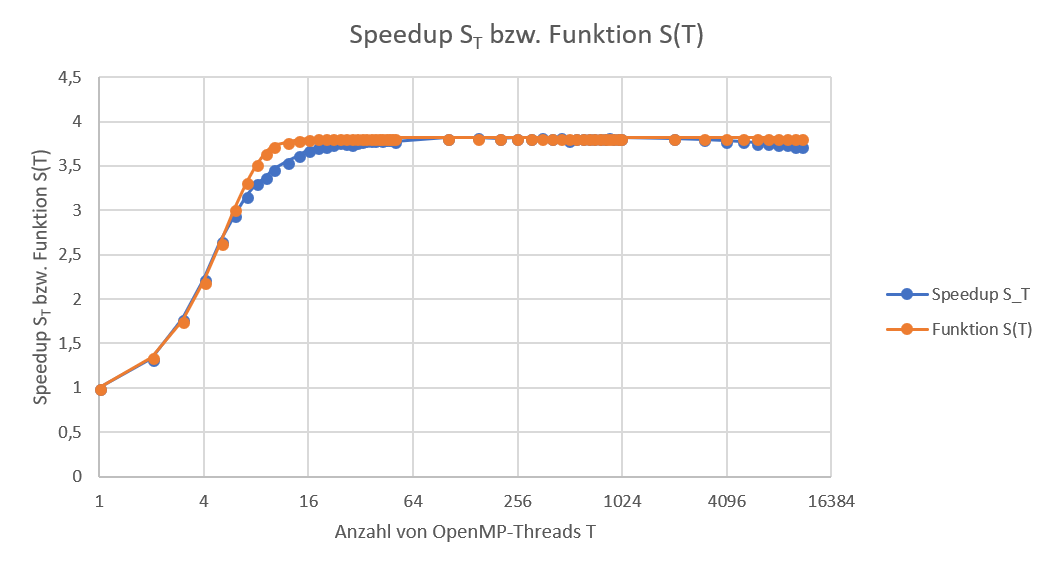
\includegraphics[width=11cm]{Abbildungen/Speedup_OpenMP_Funktion_S(t).png}
							\caption{Grafische Darstellung des Zusammenhangs zwischen dem gemessenen Speedup und der Anzahl der verwendeten OpenMP-Threads und Vergleich mit der ermittelten Funktion $S(T)$.}
							\label{fig:Speedup_OpenMP_Funktion_S(t)}
						\end{figure}
					
						Bei Vergleich des Graphen, der durch die Messung ermittelt wurde, mit dem Graphen der Näherungsfunktion $S(T)$, wird ersichtlich, dass das beobachtete Wachstum teilweise exakt mit einem logistischen Wachstum übereinstimmt. Lediglich im Bereich von 4 bis 64 OpenMP-Threads erfolgt die Abflachung bei den Messergebnissen schneller als bei der Näherungsfunktion. Auch bei sehr vielen OpenMP-Threads erkennt man, dass der Verwaltungsaufwand wiederum den Mehrwert, der durch den Einsatz von mehr OpenMP-Threads einhergeht, übersteigt, und die Speedup-Kurve langsam zu sinken beginnt.\\						
						Nun wird die Effizienz betrachtet. Sie ist in Abbildung \ref{fig:Effizienz_OpenMP} dargestellt.
						
						\begin{figure}
							\centering	
							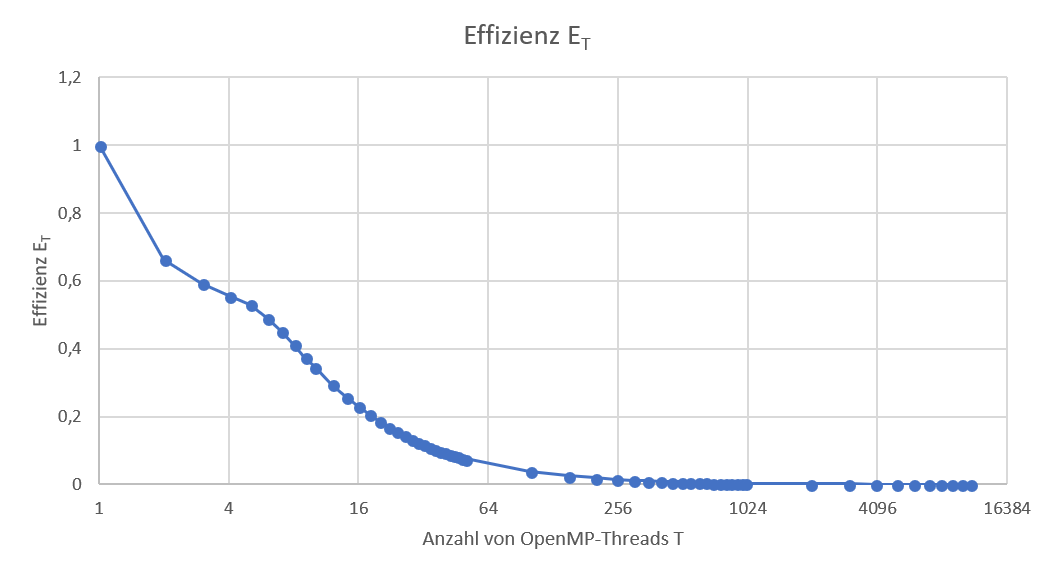
\includegraphics[width=11cm]{Abbildungen/Effizienz_OpenMP.png}
							\caption{Grafische Darstellung des Zusammenhangs zwischen der Effizienz und der Anzahl der verwendeten OpenMP-Threads.}
							\label{fig:Effizienz_OpenMP}
						\end{figure}

						Die Effizienz kommt auch in diesem Fall wieder einer stetig sinkenden Funktion gleich, welche zu Beginn drastisch sinkt und sich dann asymptotisch 0 annähert. Auch ist erkenntlich, dass die Effizienz bis ca. 16 OpenMP-Threads, wie auch aus dem Speedup-Diagramm hervorgeht, akzeptable Werte zwischen 100\% und 20\% annimmt, während sie nachher immer weiter sinkt und schließlich annähernd 0\% wird.

				\end{description}
			
				Die verschiedenen Konzepte zur parallelen Programmierung wurden nun anhand des Speedups und der Effizienz verglichen. Dies sind allerdings Größen, die Programm-Laufzeiten in Beziehung zueinander setzen und somit keine Aussage mehr über die tatsächliche Laufzeit treffen lassen. Aus diesem Grund werden in der folgenden Tabelle \ref{tab:LaufzeitVergleich} einige Laufzeiten der verschiedenen Versuche verglichen. Die erste Spalte ist mit \textit{\#} betitelt, was für \textit{Anzahl von Abarbeitungseinheiten} steht, um sowohl Prozesse, als auch Threads und die anderen Technologien unter einem allgemeinen Namen bezeichnen zu können. Die Laufzeit ist jeweils, wie bereits mehrmals erläutert, der Median aus 50 Zeit-Messungen unter denselben Bedingungen, die Bezeichner der Laufzeit-Spalten sind selbsterklärend.
				
				\begin{table}
					\caption{Laufzeit-Vergleich der parallelen Programmierkonzepte.}
					\begin{tabular}{c|c|c|c|c|c}
						\# & $t_{Seriell} [s]$ & $t_{Prozesse} [s]$ & $t_{Threads} [s]$ & $t_{MPI} [s]$ & $t_{OpenMP} [s]$\\
						\hline
						1 & 12,840 & 12,736 & 15,619 & / & 13,089\\
						2 & / & 9,743 & 11,797 & 51,612 & 9,860\\
						3 & / & 7,385 & 8,804 & 39,291 & 7,361\\
						4 & / & 5,817 & 7,084 & 29,229 & 5,890\\
						5 & / & 4,998 & 6,027 & 27,969 & 4,926\\
						6 & / & 4,454 & 5,330 & 27,920 & 4,444\\
						7 & / & 4,200 & 5,105 & 27,485 & 4,136\\
						8 & / & 3,995 & 4,868 & 27,436 & 3,963\\
						9 & / & 3,862 & 4,713 & 27,083 & 3,879\\
						10 & / & 3,803 & 4,576 & 27,119 & 3,777\\
						50 & / & 3,441 & 4,038 & 27,722 & 3,466\\
						100 & / & 3,433 & 4,034 & 28,384 & 3,431\\
						150 & / & 3,445 & 4,045 & 27,736 & 3,425\\
						200 & / & 3,433 & 4,026 & 32,170 & 3,432\\
						250 & / & 3,434 & 4,029 & 36,812 & 3,427\\
						500 & / & 3,443 & 4,042 & / & 3,457\\
						1000 & / & 3,466 & 4,047 & / & 3,428\\
						10000 & / & 3,866 & 4,382 & / & 3,510\\
						20000 & / & / & 4,827 & / & /\\
						30000 & / & / & 7,730 & / & /\\
					\end{tabular}
					\label{tab:LaufzeitVergleich}
				\end{table}
			
				Man erkennt, dass sich die Laufzeiten im Vergleich der verschiedenen Technologien kaum oder nur in wenigen Sekunden unterscheiden, nur die Laufzeiten von MPI fallen vollkommen aus dem Schema. Allerdings ist unklar, weshalb diese Laufzeiten so viel höher sind.\\
				Ein wichtiger Aspekt, der sich aus dem praktischen Teil der Arbeit in Zusammenhang mit dem Speedup ergibt, ist, dass es einen Punkt gibt, ab welchem der Verwaltungsaufwand, der mit der Erstellung einer weiteren Abarbeitungseinheit (Prozess, Thread) einhergeht, im Vergleich zum Nutzen, der mit Hilfe der hinzukommenden Abarbeitungseinheit erreicht werden kann, überwiegt und der Speedup tatsächlich ab einer großen Anzahl von Abarbeitungseinheiten wieder zu sinken beginnt.\\
				Tatsächlich war dies eine Problematik, mit welcher sich die großen Rechenzentren konfrontiert sahen. Hierbei war das Problem, dass der Kommunikationsaufwand, welcher mit einer weiteren Abarbeitungseinheit einhergeht, wächst und, dass die Bandbreiten der Verbindungsnetzwerke zu klein waren, sodass sich die Parallelisierung oft nicht lohnte. Erst vor wenigen Jahren wurde dieses Problem durch immer schneller werdende Verbindungen gelöst oder mindestens gedämpft.